\begin{frame}[t]
    \frametitle{Aufgabe 9.2 - ABBaumaßnahmen I}
    \scriptsize

    Führen Sie auf einem anfangs leeren (2, 3)-Baum die folgenden Operationen aus:

    $$
        \text{insert: } [19, 11, 28, 38, 37, 30, 7, 59, 41]
    $$

    gefolgt von:

    $$
        \text{remove: } [7, 11, 59, 19, 37, 41, 30, 38]
    $$

    \textbf{Hinweis:} Zeichnen Sie den Baum nach jedem Schritt. Sie dürfen in Ihrer Zeichnung auf
    Blattknoten verzichten.

    Beachten Sie außerdem das Folgende:

    \begin{itemize}
        \item Beim Aufspalten von Knoten während dem Einfügen wandert das Element am Index $\lfloor b/2 \rfloor$ nach oben.
        \item Beim Löschen von Elementen aus inneren Knoten wird üblicherweise versucht, entweder
              den symmetrischen Vorgänger oder symmetrischen Nachfolger intelligent zu
              wählen. Für diese Aufgabe soll darauf verzichtet werden. Stattdessen wird stets der
              symmetrische Vorgänger verwendet. Beim Stehlen von Elementen wird zunächst der
              linke Nachbar betrachtet. Beim Verschmelzen werden Knoten sofern möglich mit ihrem
              linken Nachbarn, ansonsten mit dem rechten Nachbarn, vereinigt.
    \end{itemize}

\end{frame}

% \node[spaceStyle](root_S0) at (-0.53, 0) {};
% \node[nodeStyle] (root_0)  at (    0, 0) {x};
% \node[spaceStyle](root_S1) at ( 0.53, 0) {};

% \node[spaceStyle](root_S0) at (-1.06, 0) {};
% \node[nodeStyle] (root_0)  at (-0.53, 0) {x};
% \node[spaceStyle](root_S1) at (    0, 0) {};
% \node[nodeStyle] (root_1)  at ( 0.53, 0) {y};
% \node[spaceStyle](root_S2) at ( 1.06, 0) {};

\begin{frame}[t]
    \frametitle{Aufgabe 9.2 - ABBaumaßnahmen I}
    Insert 11:
    \bigskip
    \bigskip

    \begin{columns}
        \begin{column}{0.48\textwidth}
            \begin{center}
                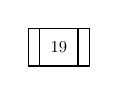
\begin{tikzpicture}[nodeStyle/.style={rectangle, draw, minimum size=0.8cm}, spaceStyle/.style={rectangle, draw, minimum width=0.2cm, minimum height=0.8cm}, scale=0.6, transform shape]
                    \node[spaceStyle](root_S0) at (-0.53, 0) {};
                    \node[nodeStyle] (root_0)  at (0, 0) {19};
                    \node[spaceStyle](root_S1) at (0.53, 0) {};
                \end{tikzpicture}
            \end{center}
        \end{column}
        \begin{column}{0.48\textwidth}
        \end{column}
    \end{columns}
\end{frame}

\begin{frame}[t]
    \frametitle{Aufgabe 9.2 - ABBaumaßnahmen I}
    Insert 28:
    \bigskip
    \bigskip

    \begin{columns}
        \begin{column}{0.48\textwidth}
            \begin{center}
                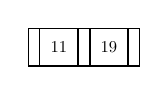
\begin{tikzpicture}[nodeStyle/.style={rectangle, draw, minimum size=0.8cm}, spaceStyle/.style={rectangle, draw, minimum width=0.2cm, minimum height=0.8cm}, scale=0.6, transform shape]
                    \node[spaceStyle](root_S0) at (-1.06, 0) {};
                    \node[nodeStyle] (root_0)  at (-0.53, 0) {11};
                    \node[spaceStyle](root_S1) at (    0, 0) {};
                    \node[nodeStyle] (root_1)  at ( 0.53, 0) {19};
                    \node[spaceStyle](root_S2) at ( 1.06, 0) {};
                \end{tikzpicture}
            \end{center}
        \end{column}
        \begin{column}{0.48\textwidth}
        \end{column}
    \end{columns}
\end{frame}

\begin{frame}[t]
    \frametitle{Aufgabe 9.2 - ABBaumaßnahmen I}
    Insert 38:
    \bigskip
    \bigskip

    \begin{columns}
        \begin{column}{0.48\textwidth}
            \begin{center}
                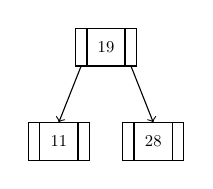
\begin{tikzpicture}[nodeStyle/.style={rectangle, draw, minimum size=0.8cm}, spaceStyle/.style={rectangle, draw, minimum width=0.2cm, minimum height=0.8cm}, scale=0.6, transform shape]
                    \node[spaceStyle](root_S0) at (-0.53, 0) {};
                    \node[nodeStyle] (root_0)  at (    0, 0) {19};
                    \node[spaceStyle](root_S1) at ( 0.53, 0) {};

                    \node[spaceStyle](11_S0) at (-0.53 - 1, -2) {};
                    \node[nodeStyle] (11_0)  at (    0 - 1, -2) {11};
                    \node[spaceStyle](11_S1) at ( 0.53 - 1, -2) {};

                    \node[spaceStyle](12_S0) at (-0.53 + 1, -2) {};
                    \node[nodeStyle] (12_0)  at (    0 + 1, -2) {28};
                    \node[spaceStyle](12_S1) at ( 0.53 + 1, -2) {};

                    \draw[->] (root_S0.south) -- (11_0.north);
                    \draw[->] (root_S1.south) -- (12_0.north);
                \end{tikzpicture}
            \end{center}
        \end{column}
        \begin{column}{0.48\textwidth}
        \end{column}
    \end{columns}
\end{frame}

\begin{frame}[t]
    \frametitle{Aufgabe 9.2 - ABBaumaßnahmen I}
    Insert 37:
    \bigskip
    \bigskip

    \begin{columns}
        \begin{column}{0.48\textwidth}
            \begin{center}
                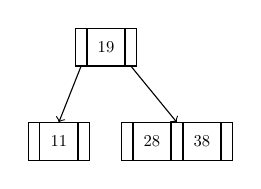
\begin{tikzpicture}[nodeStyle/.style={rectangle, draw, minimum size=0.8cm}, spaceStyle/.style={rectangle, draw, minimum width=0.2cm, minimum height=0.8cm}, scale=0.6, transform shape]
                    \node[spaceStyle](root_S0) at (-0.53, 0) {};
                    \node[nodeStyle] (root_0)  at (    0, 0) {19};
                    \node[spaceStyle](root_S1) at ( 0.53, 0) {};

                    \node[spaceStyle](11_S0) at (-0.53 - 1, -2) {};
                    \node[nodeStyle] (11_0)  at (    0 - 1, -2) {11};
                    \node[spaceStyle](11_S1) at ( 0.53 - 1, -2) {};

                    \node[spaceStyle](12_S0) at (-1.06 + 1.5, -2) {};
                    \node[nodeStyle] (12_0)  at (-0.53 + 1.5, -2) {28};
                    \node[spaceStyle](12_S1) at (    0 + 1.5, -2) {};
                    \node[nodeStyle] (12_1)  at ( 0.53 + 1.5, -2) {38};
                    \node[spaceStyle](12_S2) at ( 1.06 + 1.5, -2) {};

                    \draw[->] (root_S0.south) -- (11_0.north);
                    \draw[->] (root_S1.south) -- (12_S1.north);
                \end{tikzpicture}
            \end{center}
        \end{column}
        \begin{column}{0.48\textwidth}
        \end{column}
    \end{columns}
\end{frame}

\begin{frame}[t]
    \frametitle{Aufgabe 9.2 - ABBaumaßnahmen I}
    Insert 30:
    \bigskip
    \bigskip

    \begin{columns}
        \begin{column}{0.48\textwidth}
            \begin{center}
                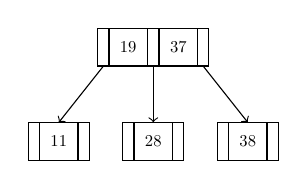
\begin{tikzpicture}[nodeStyle/.style={rectangle, draw, minimum size=0.8cm}, spaceStyle/.style={rectangle, draw, minimum width=0.2cm, minimum height=0.8cm}, scale=0.6, transform shape]
                    \node[spaceStyle](root_S0) at (-1.06, 0) {};
                    \node[nodeStyle] (root_0)  at (-0.53, 0) {19};
                    \node[spaceStyle](root_S1) at (    0, 0) {};
                    \node[nodeStyle] (root_1)  at ( 0.53, 0) {37};
                    \node[spaceStyle](root_S2) at ( 1.06, 0) {};

                    \node[spaceStyle](11_S0) at (-0.53 - 2, -2) {};
                    \node[nodeStyle] (11_0)  at (    0 - 2, -2) {11};
                    \node[spaceStyle](11_S1) at ( 0.53 - 2, -2) {};

                    \node[spaceStyle](12_S0) at (-0.53, -2) {};
                    \node[nodeStyle] (12_0)  at (    0, -2) {28};
                    \node[spaceStyle](12_S1) at ( 0.53, -2) {};

                    \node[spaceStyle](13_S0) at (-0.53 + 2, -2) {};
                    \node[nodeStyle] (13_0)  at (    0 + 2, -2) {38};
                    \node[spaceStyle](13_S1) at ( 0.53 + 2, -2) {};

                    \draw[->] (root_S0.south) -- (11_0.north);
                    \draw[->] (root_S1.south) -- (12_0.north);
                    \draw[->] (root_S2.south) -- (13_0.north);
                \end{tikzpicture}
            \end{center}
        \end{column}
        \begin{column}{0.48\textwidth}
        \end{column}
    \end{columns}
\end{frame}

\begin{frame}[t]
    \frametitle{Aufgabe 9.2 - ABBaumaßnahmen I}
    Insert 7:
    \bigskip
    \bigskip

    \begin{columns}
        \begin{column}{0.48\textwidth}
            \begin{center}
                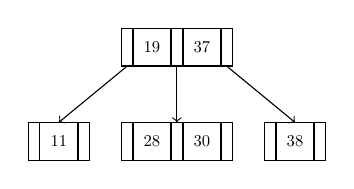
\begin{tikzpicture}[nodeStyle/.style={rectangle, draw, minimum size=0.8cm}, spaceStyle/.style={rectangle, draw, minimum width=0.2cm, minimum height=0.8cm}, scale=0.6, transform shape]
                    \node[spaceStyle](root_S0) at (-1.06, 0) {};
                    \node[nodeStyle] (root_0)  at (-0.53, 0) {19};
                    \node[spaceStyle](root_S1) at (    0, 0) {};
                    \node[nodeStyle] (root_1)  at ( 0.53, 0) {37};
                    \node[spaceStyle](root_S2) at ( 1.06, 0) {};

                    \node[spaceStyle](11_S0) at (-0.53 - 2.5, -2) {};
                    \node[nodeStyle] (11_0)  at (    0 - 2.5, -2) {11};
                    \node[spaceStyle](11_S1) at ( 0.53 - 2.5, -2) {};

                    \node[spaceStyle](12_S0) at (-1.06, -2) {};
                    \node[nodeStyle] (12_0)  at (-0.53, -2) {28};
                    \node[spaceStyle](12_S1) at (    0, -2) {};
                    \node[nodeStyle] (12_1)  at ( 0.53, -2) {30};
                    \node[spaceStyle](12_S2) at ( 1.06, -2) {};

                    \node[spaceStyle](13_S0) at (-0.53 + 2.5, -2) {};
                    \node[nodeStyle] (13_0)  at (    0 + 2.5, -2) {38};
                    \node[spaceStyle](13_S1) at ( 0.53 + 2.5, -2) {};

                    \draw[->] (root_S0.south) -- (11_0.north);
                    \draw[->] (root_S1.south) -- (12_S1.north);
                    \draw[->] (root_S2.south) -- (13_0.north);
                \end{tikzpicture}
            \end{center}
        \end{column}
        \begin{column}{0.48\textwidth}
        \end{column}
    \end{columns}
\end{frame}

\begin{frame}[t]
    \frametitle{Aufgabe 9.2 - ABBaumaßnahmen I}
    Insert 59:
    \bigskip
    \bigskip

    \begin{columns}
        \begin{column}{0.48\textwidth}
            \begin{center}
                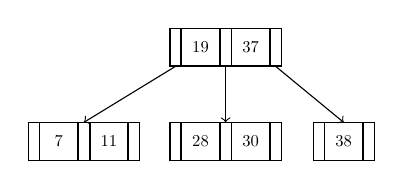
\begin{tikzpicture}[nodeStyle/.style={rectangle, draw, minimum size=0.8cm}, spaceStyle/.style={rectangle, draw, minimum width=0.2cm, minimum height=0.8cm}, scale=0.6, transform shape]
                    \node[spaceStyle](root_S0) at (-1.06, 0) {};
                    \node[nodeStyle] (root_0)  at (-0.53, 0) {19};
                    \node[spaceStyle](root_S1) at (    0, 0) {};
                    \node[nodeStyle] (root_1)  at ( 0.53, 0) {37};
                    \node[spaceStyle](root_S2) at ( 1.06, 0) {};

                    \node[spaceStyle](11_S0) at (-1.06 - 3, -2) {};
                    \node[nodeStyle] (11_0)  at (-0.53 - 3, -2) {7};
                    \node[spaceStyle](11_S1) at (    0 - 3, -2) {};
                    \node[nodeStyle] (11_1)  at ( 0.53 - 3, -2) {11};
                    \node[spaceStyle](11_S2) at ( 1.06 - 3, -2) {};

                    \node[spaceStyle](12_S0) at (-1.06, -2) {};
                    \node[nodeStyle] (12_0)  at (-0.53, -2) {28};
                    \node[spaceStyle](12_S1) at (    0, -2) {};
                    \node[nodeStyle] (12_1)  at ( 0.53, -2) {30};
                    \node[spaceStyle](12_S2) at ( 1.06, -2) {};

                    \node[spaceStyle](13_S0) at (-0.53 + 2.5, -2) {};
                    \node[nodeStyle] (13_0)  at (    0 + 2.5, -2) {38};
                    \node[spaceStyle](13_S1) at ( 0.53 + 2.5, -2) {};

                    \draw[->] (root_S0.south) -- (11_S1.north);
                    \draw[->] (root_S1.south) -- (12_S1.north);
                    \draw[->] (root_S2.south) -- (13_0.north);
                \end{tikzpicture}
            \end{center}
        \end{column}
        \begin{column}{0.48\textwidth}
        \end{column}
    \end{columns}
\end{frame}

\begin{frame}[t]
    \frametitle{Aufgabe 9.2 - ABBaumaßnahmen I}
    Insert 41:
    \bigskip
    \bigskip

    \begin{columns}
        \begin{column}{0.48\textwidth}
            \begin{center}
                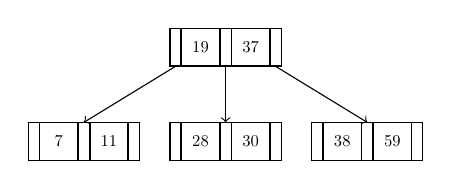
\begin{tikzpicture}[nodeStyle/.style={rectangle, draw, minimum size=0.8cm}, spaceStyle/.style={rectangle, draw, minimum width=0.2cm, minimum height=0.8cm}, scale=0.6, transform shape]
                    \node[spaceStyle](root_S0) at (-1.06, 0) {};
                    \node[nodeStyle] (root_0)  at (-0.53, 0) {19};
                    \node[spaceStyle](root_S1) at (    0, 0) {};
                    \node[nodeStyle] (root_1)  at ( 0.53, 0) {37};
                    \node[spaceStyle](root_S2) at ( 1.06, 0) {};

                    \node[spaceStyle](11_S0) at (-1.06 - 3, -2) {};
                    \node[nodeStyle] (11_0)  at (-0.53 - 3, -2) {7};
                    \node[spaceStyle](11_S1) at (    0 - 3, -2) {};
                    \node[nodeStyle] (11_1)  at ( 0.53 - 3, -2) {11};
                    \node[spaceStyle](11_S2) at ( 1.06 - 3, -2) {};

                    \node[spaceStyle](12_S0) at (-1.06, -2) {};
                    \node[nodeStyle] (12_0)  at (-0.53, -2) {28};
                    \node[spaceStyle](12_S1) at (    0, -2) {};
                    \node[nodeStyle] (12_1)  at ( 0.53, -2) {30};
                    \node[spaceStyle](12_S2) at ( 1.06, -2) {};

                    \node[spaceStyle](13_S0) at (-1.06 + 3, -2) {};
                    \node[nodeStyle] (13_0)  at (-0.53 + 3, -2) {38};
                    \node[spaceStyle](13_S1) at (    0 + 3, -2) {};
                    \node[nodeStyle] (13_1)  at ( 0.53 + 3, -2) {59};
                    \node[spaceStyle](13_S2) at ( 1.06 + 3, -2) {};

                    \draw[->] (root_S0.south) -- (11_S1.north);
                    \draw[->] (root_S1.south) -- (12_S1.north);
                    \draw[->] (root_S2.south) -- (13_S1.north);
                \end{tikzpicture}
            \end{center}
        \end{column}
        \begin{column}{0.48\textwidth}
        \end{column}
    \end{columns}
\end{frame}

\begin{frame}[t]
    \frametitle{Aufgabe 9.2 - ABBaumaßnahmen I}
    Remove 7:
    \bigskip
    \bigskip

    \begin{columns}
        \begin{column}{0.48\textwidth}
            \begin{center}
                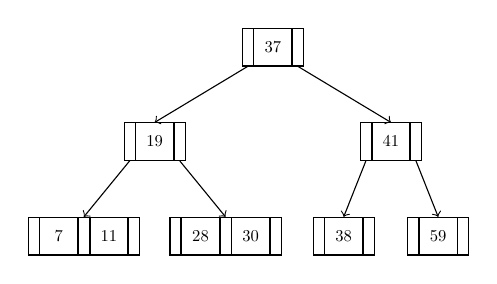
\begin{tikzpicture}[nodeStyle/.style={rectangle, draw, minimum size=0.8cm}, spaceStyle/.style={rectangle, draw, minimum width=0.2cm, minimum height=0.8cm}, scale=0.6, transform shape]
                    \node[spaceStyle](root_S0) at (-0.53, 0) {};
                    \node[nodeStyle] (root_0)  at (    0, 0) {37};
                    \node[spaceStyle](root_S1) at ( 0.53, 0) {};

                    \node[spaceStyle](11_S0) at (-0.53 - 2.5, -2) {};
                    \node[nodeStyle] (11_0)  at (    0 - 2.5, -2) {19};
                    \node[spaceStyle](11_S1) at ( 0.53 - 2.5, -2) {};

                    \node[spaceStyle](12_S0) at (-0.53 + 2.5, -2) {};
                    \node[nodeStyle] (12_0)  at (    0 + 2.5, -2) {41};
                    \node[spaceStyle](12_S1) at ( 0.53 + 2.5, -2) {};

                    \node[spaceStyle](21_S0) at (-1.06 - 4, -4) {};
                    \node[nodeStyle] (21_0)  at (-0.53 - 4, -4) {7};
                    \node[spaceStyle](21_S1) at (    0 - 4, -4) {};
                    \node[nodeStyle] (21_1)  at ( 0.53 - 4, -4) {11};
                    \node[spaceStyle](21_S2) at ( 1.06 - 4, -4) {};

                    \node[spaceStyle](22_S0) at (-1.06 - 1, -4) {};
                    \node[nodeStyle] (22_0)  at (-0.53 - 1, -4) {28};
                    \node[spaceStyle](22_S1) at (    0 - 1, -4) {};
                    \node[nodeStyle] (22_1)  at ( 0.53 - 1, -4) {30};
                    \node[spaceStyle](22_S2) at ( 1.06 - 1, -4) {};

                    \node[spaceStyle](24_S0) at (-0.53 + 1.5, -4) {};
                    \node[nodeStyle] (24_0)  at (    0 + 1.5, -4) {38};
                    \node[spaceStyle](24_S1) at ( 0.53 + 1.5, -4) {};

                    \node[spaceStyle](25_S0) at (-0.53 + 3.5, -4) {};
                    \node[nodeStyle] (25_0)  at (    0 + 3.5, -4) {59};
                    \node[spaceStyle](25_S1) at ( 0.53 + 3.5, -4) {};

                    \draw[->] (root_S0.south) -- (11_0.north);
                    \draw[->] (root_S1.south) -- (12_0.north);

                    \draw[->] (11_S0.south) -- (21_S1.north);
                    \draw[->] (11_S1.south) -- (22_S1.north);

                    \draw[->] (12_S0.south) -- (24_0.north);
                    \draw[->] (12_S1.south) -- (25_0.north);
                \end{tikzpicture}
            \end{center}
        \end{column}
        \begin{column}{0.48\textwidth}
        \end{column}
    \end{columns}
\end{frame}

\begin{frame}[t]
    \frametitle{Aufgabe 9.2 - ABBaumaßnahmen I}
    Remove 11:
    \bigskip
    \bigskip

    \begin{columns}
        \begin{column}{0.48\textwidth}
            \begin{center}
                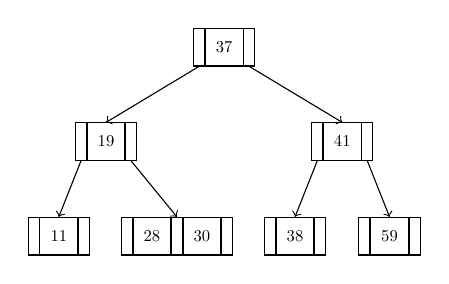
\begin{tikzpicture}[nodeStyle/.style={rectangle, draw, minimum size=0.8cm}, spaceStyle/.style={rectangle, draw, minimum width=0.2cm, minimum height=0.8cm}, scale=0.6, transform shape]
                    \node[spaceStyle](root_S0) at (-0.53, 0) {};
                    \node[nodeStyle] (root_0)  at (    0, 0) {37};
                    \node[spaceStyle](root_S1) at ( 0.53, 0) {};

                    \node[spaceStyle](11_S0) at (-0.53 - 2.5, -2) {};
                    \node[nodeStyle] (11_0)  at (    0 - 2.5, -2) {19};
                    \node[spaceStyle](11_S1) at ( 0.53 - 2.5, -2) {};

                    \node[spaceStyle](12_S0) at (-0.53 + 2.5, -2) {};
                    \node[nodeStyle] (12_0)  at (    0 + 2.5, -2) {41};
                    \node[spaceStyle](12_S1) at ( 0.53 + 2.5, -2) {};

                    \node[spaceStyle](21_S0) at (-0.53 - 3.5, -4) {};
                    \node[nodeStyle] (21_0)  at (    0 - 3.5, -4) {11};
                    \node[spaceStyle](21_S1) at ( 0.53 - 3.5, -4) {};

                    \node[spaceStyle](22_S0) at (-1.06 - 1, -4) {};
                    \node[nodeStyle] (22_0)  at (-0.53 - 1, -4) {28};
                    \node[spaceStyle](22_S1) at (    0 - 1, -4) {};
                    \node[nodeStyle] (22_1)  at ( 0.53 - 1, -4) {30};
                    \node[spaceStyle](22_S2) at ( 1.06 - 1, -4) {};

                    \node[spaceStyle](24_S0) at (-0.53 + 1.5, -4) {};
                    \node[nodeStyle] (24_0)  at (    0 + 1.5, -4) {38};
                    \node[spaceStyle](24_S1) at ( 0.53 + 1.5, -4) {};

                    \node[spaceStyle](25_S0) at (-0.53 + 3.5, -4) {};
                    \node[nodeStyle] (25_0)  at (    0 + 3.5, -4) {59};
                    \node[spaceStyle](25_S1) at ( 0.53 + 3.5, -4) {};

                    \draw[->] (root_S0.south) -- (11_0.north);
                    \draw[->] (root_S1.south) -- (12_0.north);

                    \draw[->] (11_S0.south) -- (21_0.north);
                    \draw[->] (11_S1.south) -- (22_S1.north);

                    \draw[->] (12_S0.south) -- (24_0.north);
                    \draw[->] (12_S1.south) -- (25_0.north);
                \end{tikzpicture}
            \end{center}
        \end{column}
        \begin{column}{0.48\textwidth}
        \end{column}
    \end{columns}
\end{frame}

\begin{frame}[t]
    \frametitle{Aufgabe 9.2 - ABBaumaßnahmen I}
    Remove 59:
    \bigskip
    \bigskip

    \begin{columns}
        \begin{column}{0.48\textwidth}
            \begin{center}
                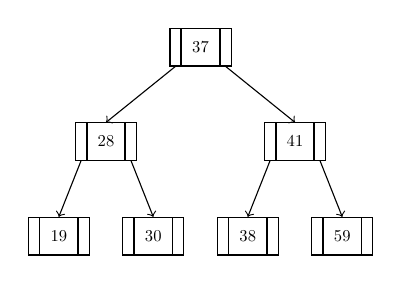
\begin{tikzpicture}[nodeStyle/.style={rectangle, draw, minimum size=0.8cm}, spaceStyle/.style={rectangle, draw, minimum width=0.2cm, minimum height=0.8cm}, scale=0.6, transform shape]
                    \node[spaceStyle](root_S0) at (-0.53, 0) {};
                    \node[nodeStyle] (root_0)  at (    0, 0) {37};
                    \node[spaceStyle](root_S1) at ( 0.53, 0) {};

                    \node[spaceStyle](11_S0) at (-0.53 - 2, -2) {};
                    \node[nodeStyle] (11_0)  at (    0 - 2, -2) {28};
                    \node[spaceStyle](11_S1) at ( 0.53 - 2, -2) {};

                    \node[spaceStyle](12_S0) at (-0.53 + 2, -2) {};
                    \node[nodeStyle] (12_0)  at (    0 + 2, -2) {41};
                    \node[spaceStyle](12_S1) at ( 0.53 + 2, -2) {};

                    \node[spaceStyle](21_S0) at (-0.53 - 3, -4) {};
                    \node[nodeStyle] (21_0)  at (    0 - 3, -4) {19};
                    \node[spaceStyle](21_S1) at ( 0.53 - 3, -4) {};

                    \node[spaceStyle](22_S0) at (-0.53 - 1, -4) {};
                    \node[nodeStyle] (22_0)  at (    0 - 1, -4) {30};
                    \node[spaceStyle](22_S1) at ( 0.53 - 1, -4) {};

                    \node[spaceStyle](24_S0) at (-0.53 + 1, -4) {};
                    \node[nodeStyle] (24_0)  at (    0 + 1, -4) {38};
                    \node[spaceStyle](24_S1) at ( 0.53 + 1, -4) {};

                    \node[spaceStyle](25_S0) at (-0.53 + 3, -4) {};
                    \node[nodeStyle] (25_0)  at (    0 + 3, -4) {59};
                    \node[spaceStyle](25_S1) at ( 0.53 + 3, -4) {};

                    \draw[->] (root_S0.south) -- (11_0.north);
                    \draw[->] (root_S1.south) -- (12_0.north);

                    \draw[->] (11_S0.south) -- (21_0.north);
                    \draw[->] (11_S1.south) -- (22_0.north);

                    \draw[->] (12_S0.south) -- (24_0.north);
                    \draw[->] (12_S1.south) -- (25_0.north);
                \end{tikzpicture}
            \end{center}
        \end{column}
        \begin{column}{0.48\textwidth}
        \end{column}
    \end{columns}
\end{frame}

\begin{frame}[t]
    \frametitle{Aufgabe 9.2 - ABBaumaßnahmen I}
    Remove 19:
    \bigskip
    \bigskip

    \begin{columns}
        \begin{column}{0.48\textwidth}
            \begin{center}
                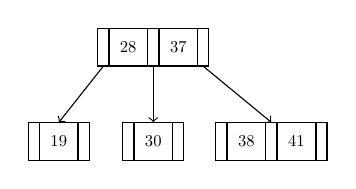
\begin{tikzpicture}[nodeStyle/.style={rectangle, draw, minimum size=0.8cm}, spaceStyle/.style={rectangle, draw, minimum width=0.2cm, minimum height=0.8cm}, scale=0.6, transform shape]
                    \node[spaceStyle](root_S0) at (-1.06, 0) {};
                    \node[nodeStyle] (root_0)  at (-0.53, 0) {28};
                    \node[spaceStyle](root_S1) at (    0, 0) {};
                    \node[nodeStyle] (root_1)  at ( 0.53, 0) {37};
                    \node[spaceStyle](root_S2) at ( 1.06, 0) {};

                    \node[spaceStyle](11_S0) at (-0.53 - 2, -2) {};
                    \node[nodeStyle] (11_0)  at (    0 - 2, -2) {19};
                    \node[spaceStyle](11_S1) at ( 0.53 - 2, -2) {};

                    \node[spaceStyle](12_S0) at (-0.53, -2) {};
                    \node[nodeStyle] (12_0)  at (    0, -2) {30};
                    \node[spaceStyle](12_S1) at ( 0.53, -2) {};

                    \node[spaceStyle](13_S0) at (-1.06 + 2.5, -2) {};
                    \node[nodeStyle] (13_0)  at (-0.53 + 2.5, -2) {38};
                    \node[spaceStyle](13_S1) at (    0 + 2.5, -2) {};
                    \node[nodeStyle] (13_1)  at ( 0.53 + 2.5, -2) {41};
                    \node[spaceStyle](13_S2) at ( 1.06 + 2.5, -2) {};

                    \draw[->] (root_S0.south) -- (11_0.north);
                    \draw[->] (root_S1.south) -- (12_0.north);
                    \draw[->] (root_S2.south) -- (13_S1.north);
                \end{tikzpicture}
            \end{center}
        \end{column}
        \begin{column}{0.48\textwidth}
        \end{column}
    \end{columns}
\end{frame}

\begin{frame}[t]
    \frametitle{Aufgabe 9.2 - ABBaumaßnahmen I}
    Remove 37:
    \bigskip
    \bigskip

    \begin{columns}
        \begin{column}{0.48\textwidth}
            \begin{center}
                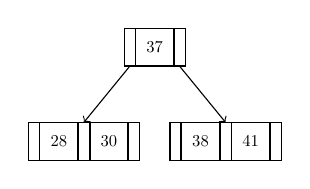
\begin{tikzpicture}[nodeStyle/.style={rectangle, draw, minimum size=0.8cm}, spaceStyle/.style={rectangle, draw, minimum width=0.2cm, minimum height=0.8cm}, scale=0.6, transform shape]
                    \node[spaceStyle](root_S0) at (-0.53, 0) {};
                    \node[nodeStyle] (root_0)  at (    0, 0) {37};
                    \node[spaceStyle](root_S1) at ( 0.53, 0) {};

                    \node[spaceStyle](11_S0) at (-1.06 - 1.5, -2) {};
                    \node[nodeStyle] (11_0)  at (-0.53 - 1.5, -2) {28};
                    \node[spaceStyle](11_S1) at (    0 - 1.5, -2) {};
                    \node[nodeStyle] (11_1)  at ( 0.53 - 1.5, -2) {30};
                    \node[spaceStyle](11_S2) at ( 1.06 - 1.5, -2) {};

                    \node[spaceStyle](12_S0) at (-1.06 + 1.5, -2) {};
                    \node[nodeStyle] (12_0)  at (-0.53 + 1.5, -2) {38};
                    \node[spaceStyle](12_S1) at (    0 + 1.5, -2) {};
                    \node[nodeStyle] (12_1)  at ( 0.53 + 1.5, -2) {41};
                    \node[spaceStyle](12_S2) at ( 1.06 + 1.5, -2) {};

                    \draw[->] (root_S0.south) -- (11_S1.north);
                    \draw[->] (root_S1.south) -- (12_S1.north);
                \end{tikzpicture}
            \end{center}
        \end{column}
        \begin{column}{0.48\textwidth}
        \end{column}
    \end{columns}
\end{frame}

\begin{frame}[t]
    \frametitle{Aufgabe 9.2 - ABBaumaßnahmen I}
    Remove 41:
    \bigskip
    \bigskip

    \begin{columns}
        \begin{column}{0.48\textwidth}
            \begin{center}
                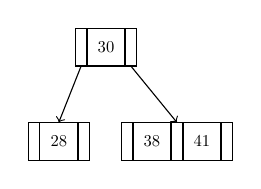
\begin{tikzpicture}[nodeStyle/.style={rectangle, draw, minimum size=0.8cm}, spaceStyle/.style={rectangle, draw, minimum width=0.2cm, minimum height=0.8cm}, scale=0.6, transform shape]
                    \node[spaceStyle](root_S0) at (-0.53, 0) {};
                    \node[nodeStyle] (root_0)  at (    0, 0) {30};
                    \node[spaceStyle](root_S1) at ( 0.53, 0) {};

                    \node[spaceStyle](11_S0) at (-0.53 - 1, -2) {};
                    \node[nodeStyle] (11_0)  at (    0 - 1, -2) {28};
                    \node[spaceStyle](11_S1) at ( 0.53 - 1, -2) {};

                    \node[spaceStyle](12_S0) at (-1.06 + 1.5, -2) {};
                    \node[nodeStyle] (12_0)  at (-0.53 + 1.5, -2) {38};
                    \node[spaceStyle](12_S1) at (    0 + 1.5, -2) {};
                    \node[nodeStyle] (12_1)  at ( 0.53 + 1.5, -2) {41};
                    \node[spaceStyle](12_S2) at ( 1.06 + 1.5, -2) {};

                    \draw[->] (root_S0.south) -- (11_0.north);
                    \draw[->] (root_S1.south) -- (12_S1.north);
                \end{tikzpicture}
            \end{center}
        \end{column}
        \begin{column}{0.48\textwidth}
        \end{column}
    \end{columns}
\end{frame}

\begin{frame}[t]
    \frametitle{Aufgabe 9.2 - ABBaumaßnahmen I}
    Remove 30:
    \bigskip
    \bigskip

    \begin{columns}
        \begin{column}{0.48\textwidth}
            \begin{center}
                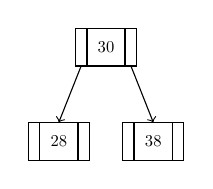
\begin{tikzpicture}[nodeStyle/.style={rectangle, draw, minimum size=0.8cm}, spaceStyle/.style={rectangle, draw, minimum width=0.2cm, minimum height=0.8cm}, scale=0.6, transform shape]
                    \node[spaceStyle](root_S0) at (-0.53, 0) {};
                    \node[nodeStyle] (root_0)  at (    0, 0) {30};
                    \node[spaceStyle](root_S1) at ( 0.53, 0) {};

                    \node[spaceStyle](11_S0) at (-0.53 - 1, -2) {};
                    \node[nodeStyle] (11_0)  at (    0 - 1, -2) {28};
                    \node[spaceStyle](11_S1) at ( 0.53 - 1, -2) {};

                    \node[spaceStyle](12_S0) at (-0.53 + 1, -2) {};
                    \node[nodeStyle] (12_0)  at (    0 + 1, -2) {38};
                    \node[spaceStyle](12_S1) at ( 0.53 + 1, -2) {};

                    \draw[->] (root_S0.south) -- (11_0.north);
                    \draw[->] (root_S1.south) -- (12_0.north);
                \end{tikzpicture}
            \end{center}
        \end{column}
        \begin{column}{0.48\textwidth}
        \end{column}
    \end{columns}
\end{frame}

\begin{frame}[t]
    \frametitle{Aufgabe 9.2 - ABBaumaßnahmen I}
    Remove 38:
    \bigskip
    \bigskip

    \begin{columns}
        \begin{column}{0.48\textwidth}
            \begin{center}
                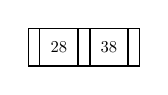
\begin{tikzpicture}[nodeStyle/.style={rectangle, draw, minimum size=0.8cm}, spaceStyle/.style={rectangle, draw, minimum width=0.2cm, minimum height=0.8cm}, scale=0.6, transform shape]
                    \node[spaceStyle](root_S0) at (-1.06, 0) {};
                    \node[nodeStyle] (root_0)  at (-0.53, 0) {28};
                    \node[spaceStyle](root_S1) at (    0, 0) {};
                    \node[nodeStyle] (root_1)  at ( 0.53, 0) {38};
                    \node[spaceStyle](root_S2) at ( 1.06, 0) {};
                \end{tikzpicture}
            \end{center}
        \end{column}
        \begin{column}{0.48\textwidth}
        \end{column}
    \end{columns}
\end{frame}

\begin{frame}[t]
    \frametitle{Aufgabe 9.2 - ABBaumaßnahmen I (Extra Platz)}
\end{frame}